
\begin{figure}[t]
%  \centerline {
    \begin{subfigure}{0.40\textwidth}
      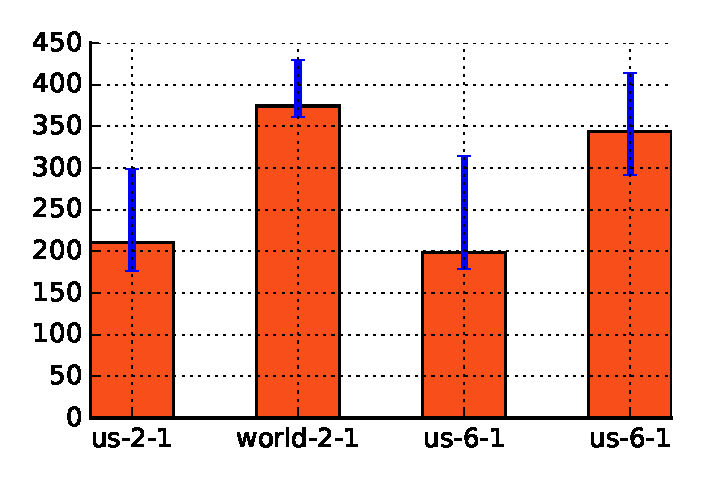
\includegraphics[width=\linewidth]{plots/giza_four_put}

      % \placeholder{
      %   x-axis: \# clients / partition\\
      %   y-axis: cluster throughput\\
      %   lines: \name{}, OCC, 2PL, TAPIR\\
      %   }
%                \vspace{-1\baselineskip}
      \caption{Put}
      \label{fig:eval_giza_put_four}
    \end{subfigure}
%    \begin{subfigure}{0.33\textwidth}
%      \includegraphics[width=\linewidth]{figs/graphs/multi_dc/tpcc/tpcc_NEW_ORDER_tpcc_client_lat90.eps}
%
%      % \placeholder{
%      %   x-axis: \# clients / partition\\
%      %   y-axis: latency (median, p90, p99)\\
%      %   (maybe only show median and p99 or just median and report typical distribution)\\
%      %   lines: \name{}, OCC, 2PL, TAPIR\\
%      % }
%      \caption{90\% Latency}
%      \label{fig:geo_tpcc_latency}
%    \end{subfigure}
    \begin{subfigure}{0.40\textwidth}
      \includegraphics[width=\linewidth]{plots/giza_four_get}

      % \placeholder{
      %   x-axis: \# clients / partition\\
      %   y-axis: commit rate\\
      %   lines: \name{}, OCC, 2PL, TAPIR\\
      % }
      %\includegraphics[width=\linewidth]{fig/kodiak/tpcc_mix_10_nlog_ct_cr.pdf}
%                \vspace{-1\baselineskip}
      \caption{Get}
      \label{fig:eval_giza_get_four}
    \end{subfigure}
%  }
  \caption{Performance for \name in different setups}
\end{figure}

%%% Local Variables:
%%% mode: latex
%%% TeX-master: "main"
%%% End:
